%! Author = Bernát
%! Date = 2025. 10. 29.
% LaTeX mintafájl szakdolgozat és diplomamunkáknak az
% SZTE Informatikai Tanszekcsoportja által megkövetelt
% formai követelményeinek megvalósításához
% Modositva: 2011.04.28 Nemeth L. Zoltan
% A fájl használatához szükséges a magyar.ldf 2005/05/12 v1.5-ös vagy késõbbi verziója
% ez letölthetõ a http://www.math.bme.hu/latex/ weblapról, a magyar nyelvû szedéshez
% Hasznos információk, linekek, LaTeX leirasok a www.latex.lap.hu weboldalon vannak.
%


\documentclass[12pt]{report}

%Magyar nyelvi támogatás (Babel 3.7 vagy késõbbi kell!)
\usepackage[utf8]{inputenc}
\usepackage{t1enc}
\usepackage[magyar]{babel}
% A formai kovetelmenyekben megkövetelt Times betûtípus hasznalata:
\usepackage{times}

%Az AMS csomagjai
\usepackage{amsmath}
\usepackage{amssymb}
\usepackage{amsthm}

%A fejléc láblécek kialakításához:
\usepackage{fancyhdr}

%Természetesen további csomagok is használhatók,
%például ábrák beillesztéséhez a graphix és a psfrag,
%ha nincs rájuk szükség természetesen kihagyhatók.
\usepackage{graphicx}
\usepackage{psfrag}

% saját csomagok
\usepackage{hyperref}

%tetelszerû környezetek definiálhatók, ezek most fejezetenkent egyutt szamozodnak, pl.
\newtheorem{tet}{tetel}[chapter]
\newtheorem{defi}[tet]{Definíció}
\newtheorem{lemma}[tet]{Lemma}
\newtheorem{áll}[tet]{Állítás}
\newtheorem{köv}[tet]{Következmény}

%Ha a megjegyzések és a példak szövegét nem akarjuk dõlten szedni, akkor
%az alábbi parancs után kell õket definiální:
\theoremstyle{definition}
\newtheorem{megj}[tet]{Megjegyzés}
\newtheorem{pld}[tet]{Példa}

%Margók:
\hoffset -1in
\voffset -1in
\oddsidemargin 35mm
\textwidth 150mm
\topmargin 15mm
\headheight 10mm
\headsep 5mm
\textheight 237mm



% Document
\begin{document}

%A FEJEZETEK KEZDÕOLDALAINAK FEJ ES LÁBLÉCE:
%a plain oldalstílust kell átdefiniálni, hogy ott ne legyen fejléc:
\fancypagestyle{plain}{%
%ez mindent töröl:
\fancyhf{}
% a láblécbe jobboldalra kerüljön az oldalszám:
\fancyfoot[R]{\thepage}
%elválasztó vonal sem kell:
\renewcommand{\headrulewidth}{0pt}
}

%A TÖBBI OLDAL FEJ ÉS LÁBLÉCE:
\pagestyle{fancy}
\fancyhf{}
\fancyhead[L]{A nagy nyelvi modellek szemantikus képességeinek konzisztenciájának vizsgálata}
\fancyfoot[R]{\thepage}


%A címoldalra se fej- se lábléc nem kell:
\thispagestyle{empty}

\begin{center}
\vspace*{1cm}
{\Large\bf Szegedi Tudományegyetem}

\vspace{0.5cm}

{\Large\bf Informatikai Intézet}

\vspace*{3.8cm}


{\LARGE\bf A nagy nyelvi modellek szemantikus képességeinek konzisztenciájának vizsgálata}

{\LARGE\bf Analyzing the Consistency of Semantical Capabilities of Large Language Models}

\vspace*{3.6cm}

{\Large Diplomamunka}
% vagy {\Large Szakdolgozat}

\vspace*{4cm}

%Értelemszerûen megváltoztatandó:
{\large
\begin{tabular}{c@{\hspace{4cm}}c}
\emph{Készítette:}     &\emph{Témavezetõ:}\\
\bf{Fábián Bernát}  &\bf{Dr. Berend Gábor Iván}\\
informatika szakos     &egyetemi docens\\
hallgató&
\end{tabular}
}

\vspace*{2.3cm}

{\Large
Szeged
\\
\vspace{2mm}
2011
}
\end{center}


%A tartalomjegyzék:
\tableofcontents

%A \chapter* parancs nem ad a fejezetnek sorszámot
\chapter*{Feladatkiírás}
%A tartalomjegyzékben mégis szerepeltetni kell, mint szakasz(section) szerepeljen:
\addcontentsline{toc}{section}{Feladatkiírás}


A hallgató feladata egy olyan keretrendszer megvalósítása, amely lehetővé teszi a nagy nyelvi modellek szemantikával kapcsolatos képességeinek konzisztenciájának vizsgálatát. A kiértékelés során azt vizsgálja a keretrendszer, hogy a nagy nyelvi modellek válaszai milyen érzékenységet mutatnak olyan invarianciákra, amelyek az emberi válaszadásra nincsenek befolyással. A kísérletek során a nagy nyelvi modellek azzal kapcsolatos érzékenységének vizsgálata a cél, hogy mennyiben érzékenyek a nagy nyelvi modellek a Word-in-Context nevű feladat megoldása során az egyes inputokban szereplő mondatpárosok sorrendjének megcserélésére.

\chapter*{Tartalmi összefoglaló}
\addcontentsline{toc}{section}{Tartalmi összefoglaló}

A tartalmi összefoglalónak tartalmaznia kell (rövid, legfeljebb egy oldalas, összefüggõ megfogalmazásban)
a következõket: a téma megnevezése, a megadott feladat megfogalmazása - a feladatkiíráshoz viszonyítva-,
a megoldási mód, az alkalmazott eszközök, módszerek, az elért eredmények, kulcsszavak (4-6 darab).

Az összefoglaló nyelvének meg kell egyeznie a dolgozat nyelvével. Ha a dolgozat idegen nyelven készül,
magyar nyelvû tartalmi összefoglaló készítése is kötelezõ (külön lapon), melynek terjedelmét a TVSZ szabályozza.


 \textbf{A téma megnevezése}
    A nagy nyelvi modellek szemantikus
képességeinek konzisztenciájának vizsgálata.

\textbf{A feladat megfogalmazása}
    A használandó adathalmaz a \href{Word-in-Context dataset}{}. A kérdéseket egyenes és fordított sorrendben is fel kell tenni a modelleknek, majd összehasonlítani a válaszaikat az azonos tartalmú, de felcserélt szósorrendű kérdésekre, ezzel felmérve a szemantikus képességeiket és nyelvi konzisztenciájukat. Ez egy, az embernek könnyű, de a modellek számára problémát okozó feladat.

 \textbf{A megoldási mód}
    Hugging Face nyelvi modellek futtatása az előre meghatározott adathalmaz (Word-in-Context) kérdéseire.

    A program inputja tetszőleges sornyi bejegyzés a Word-in-Context adathalmaz 'test' splitjéből, (vagy tetszőleges, ezzel megegyező formátumú kérdéshalmaz), és tetszőleges modell a Hugging Face platformról.

    % A megoldásom során törekedtem arra, hogy az bárki által reprodukálható legyen, ezért ingyenesen elérhető és nyílt forráskódú eszközöket (Python, GitHub, Hugging Face) használtam.
    %   \begin{itemize}
    %     \item
    %           A szakdolgozatom első felében kielemeztem az eddigi legjobb modelleket és a legjobb módszereket szójelentés-értelmezés szempontjából és nyílt forráskódú nyelvi modelleket kerestem a LMArena és Hugging Face felületein, továbbá az utóbbiak futtatásának dokumentációját tanulmányoztam.
    %         \item Összehasonlító teljesítményvizsgálatot végeztem a
    %         % TODO update-elni Gemma3-ra és QWEN3-ra mindenhol
    %         \href{https://huggingface.co/microsoft/Phi-4-mini-instruct}{Phi-4-mini-instruct}, \href{https://huggingface.co/google/gemma-2-2b-it}{Gemma-2-2b-it} és a \href{https://huggingface.co/Qwen/Qwen1.5-1.8B-Chat}{Qwen1.5-1.8B-Chat} között egy Google Colab szkriptben.
    %     \item
    %           Saját adatfeldolgozó kiértékelő Python modult készítettem a promptolás automatizálásához és a modell válaszok feldolgozására.
    %     \item A választott modelleket inferenciára bírtam az automatizáló szkriptekkel különböző módokban a szósorrend-érzékenységének és egyéb metrikák összehasonlítására

      % \end{itemize}
 \textbf{Az alkalmazott eszközök, módszerek}
        Alkalmazott eszközök:
      \begin{itemize}

        \item Google Colab és PyCharm, Python futtatókörnyezet
        \item Git, GitHub
        \item Hugging Face
        \item Torch és Transformers Python könyvtárak
        \item NLTK és WordNet
        \item CUDA, Accelerate, x\_hf Python könyvtárak

      \end{itemize},

        Alkalmazott módszerek:
      \begin{itemize}

        \item Objektum Orientált Python programozás
        \item Clean Code alapelvek Martin és Robert Clean Code c. könyve \cite{martin2008cleancode} alapján

      \end{itemize}

  \textbf{Elért eredmények}

 \textbf{Kulcsszavak}
        \\
       Nagy nyelvi modell, Word-in-Context, nyelvi konzisztencia, teljesítmény-összehasonlítás

\chapter*{Motiváció}
\addcontentsline{toc}{section}{Motiváció}

Az informatika és a nyelvtechnológia fejlődésével a generatív mesterséges intelligencia mindennapjaink részévé vált. A nagy nyelvi modellek kiértékelésére számos
benchmark, azaz teljesítményteszt, metrika fejlődött ki az évek során. A legnépszer˝ubb ˝
ilyen benchmark a SuperGLUE Benchmark, amely 8, komoly kihívást jelento feladat elé ˝
állítja a nagy nyelvi modelleket. Ebben a papírban a WiC feladatot mutatom be.
A WiC (Word-in-Context) probléma a SuperGlue 8 feladatának egyike. Az emberi
szöveget érto nyelvi modellek fejlesztése kiemelten fontos mind az akadémiai kutatásban, mind a gyakorlati alkalmazásokban. Az angol nyelv˝u szövegek feldolgozása nem
csak az angolszász területeken releváns, hanem Magyarországon is, hiszen az angol nyelv
használata a számítógépek világában mindennapjaink része. Az egyetem és a helyi vállalatok is aktívan foglalkoznak természetesnyelv-feldolgozási (NLP) megoldásokkal. A
munkahelyeken – különösen IT területen – egy jól m˝uködo WiC modell jelent ˝ os el ˝ onyt ˝
biztosíthat kódok, dokumentumok, ügyfélkommunikáció vagy akár jogi szövegek értelmezésében, ami kulcsfontosságú lehet például a tudásközpontokban és startup cégeknél
is. Egy hatékony WiC modell tehát nemcsak tudományos értékkel bír, hanem gyakorlati
alkalmazásokban is közvetlen hasznot hozhat, foleg a nyelvészeti informatikai területen dolgozók számára.


\chapter{Egy találó cím}

Ez pedig már az elsõ fejezet, ...

\section{Alcím}
Ebben alfejezetek is lehetnek

\subsection{Al-al cím}
Sõt al-al fejezetek is.

\subsection{Másik}
Na lássunk egy másodikat is.

\subsection{Harmadik}
Meg egy harmadikat is.

\section{Mindjárt vége a fejezetnek}
Tényleg, itt valóban vége.


\chapter{Hosszú}
\section{Részletek}
Ebbe a fejezetbe pedig írunk sok sok szöveget. Szöveg, szöveg, szöveg,  szöveg, szöveg, szöveg,   szöveg, szöveg, szöveg
szöveg, szöveg, szöveg,  szöveg, szöveg, szöveg, szöveg, szöveg, szöveg, szöveg, szöveg, szöveg, szöveg, szöveg, szöveg,
szöveg, szöveg, szöveg, szöveg, szöveg, szöveg, szöveg, szöveg, szöveg, szöveg, szöveg, szöveg, szöveg, szöveg, szöveg,
szöveg, szöveg, szöveg, szöveg, szöveg, szöveg, szöveg, szöveg, szöveg, szöveg, szöveg, szöveg,
szöveg, szöveg, szöveg, szöveg, szöveg, szöveg, szöveg, szöveg, szöveg, szöveg, szöveg, szöveg, szöveg, szöveg, szöveg,
szöveg, szöveg, szöveg, szöveg, szöveg, szöveg, szöveg, szöveg, szöveg, szöveg, szöveg, szöveg, szöveg, szöveg, szöveg,
szöveg, szöveg, szöveg, szöveg, szöveg, szöveg, szöveg, szöveg, szöveg, szöveg, szöveg, szöveg, szöveg, szöveg, szöveg,
szöveg, szöveg, szöveg, szöveg, szöveg, szöveg, szöveg, szöveg, szöveg, szöveg, szöveg, szöveg, szöveg, szöveg, szöveg,
szöveg, szöveg, szöveg, szöveg, szöveg, szöveg, szöveg, szöveg, szöveg, szöveg, szöveg, szöveg, szöveg, szöveg, szöveg,
szöveg, szöveg, szöveg, szöveg, szöveg, szöveg, szöveg, szöveg, szöveg, szöveg, szöveg, szöveg, szöveg, szöveg, szöveg,
szöveg, szöveg, szöveg, szöveg, szöveg, szöveg, szöveg, szöveg, szöveg, szöveg, szöveg, szöveg, szöveg, szöveg, szöveg,
szöveg, szöveg, szöveg,  szöveg, szöveg, szöveg, szöveg, szöveg, szöveg, szöveg, szöveg, szöveg, szöveg, szöveg, szöveg,
szöveg, szöveg, szöveg, szöveg, szöveg, szöveg, szöveg, szöveg, szöveg, szöveg, szöveg, szöveg, szöveg, szöveg, szöveg,
szöveg, szöveg, szöveg, szöveg, szöveg, szöveg, szöveg, szöveg, szöveg, szöveg, szöveg, szöveg,
szöveg, szöveg, szöveg, szöveg, szöveg, szöveg, szöveg, szöveg, szöveg, szöveg, szöveg, szöveg, szöveg, szöveg, szöveg,
szöveg, szöveg, szöveg, szöveg, szöveg, szöveg, szöveg, szöveg, szöveg, szöveg, szöveg, szöveg, szöveg, szöveg, szöveg,
szöveg, szöveg, szöveg, szöveg, szöveg, szöveg, szöveg, szöveg, szöveg, szöveg, szöveg, szöveg, szöveg, szöveg, szöveg,
szöveg, szöveg, szöveg, szöveg, szöveg, szöveg, szöveg, szöveg, szöveg, szöveg, szöveg, szöveg, szöveg, szöveg, szöveg,
szöveg, szöveg, szöveg, szöveg, szöveg, szöveg, szöveg, szöveg, szöveg, szöveg, szöveg, szöveg, szöveg, szöveg, szöveg,
szöveg, szöveg, szöveg, szöveg, szöveg, szöveg, szöveg, szöveg, szöveg, szöveg, szöveg, szöveg, szöveg, szöveg, szöveg,
szöveg, szöveg, szöveg, szöveg, szöveg, szöveg, szöveg, szöveg, szöveg, szöveg, szöveg, szöveg, szöveg, szöveg, szöveg,
szöveg, szöveg, szöveg,  szöveg, szöveg, szöveg, szöveg, szöveg, szöveg, szöveg, szöveg, szöveg, szöveg, szöveg, szöveg,
szöveg, szöveg, szöveg, szöveg, szöveg, szöveg, szöveg, szöveg, szöveg, szöveg, szöveg, szöveg, szöveg, szöveg, szöveg,
szöveg, szöveg, szöveg, szöveg, szöveg, szöveg, szöveg, szöveg, szöveg, szöveg, szöveg, szöveg,
szöveg, szöveg, szöveg, szöveg, szöveg, szöveg, szöveg, szöveg, szöveg, szöveg, szöveg, szöveg, szöveg, szöveg, szöveg,
szöveg, szöveg, szöveg, szöveg, szöveg, szöveg, szöveg, szöveg, szöveg, szöveg, szöveg, szöveg, szöveg, szöveg, szöveg,
szöveg, szöveg, szöveg, szöveg, szöveg, szöveg, szöveg, szöveg, szöveg, szöveg, szöveg, szöveg, szöveg, szöveg, szöveg,
szöveg, szöveg, szöveg, szöveg, szöveg, szöveg, szöveg, szöveg, szöveg, szöveg, szöveg, szöveg, szöveg, szöveg, szöveg,
szöveg, szöveg, szöveg, szöveg, szöveg, szöveg, szöveg, szöveg, szöveg, szöveg, szöveg, szöveg, szöveg, szöveg, szöveg,
szöveg, szöveg, szöveg, szöveg, szöveg, szöveg, szöveg, szöveg, szöveg, szöveg, szöveg, szöveg, szöveg, szöveg, szöveg,
szöveg, szöveg, szöveg, szöveg, szöveg, szöveg, szöveg, szöveg, szöveg, szöveg, szöveg, szöveg, szöveg, szöveg, szöveg,
szöveg, szöveg, szöveg,  szöveg, szöveg, szöveg, szöveg, szöveg, szöveg, szöveg, szöveg, szöveg, szöveg, szöveg, szöveg,
szöveg, szöveg, szöveg, szöveg, szöveg, szöveg, szöveg, szöveg, szöveg, szöveg, szöveg, szöveg, szöveg, szöveg, szöveg,
szöveg, szöveg, szöveg, szöveg, szöveg, szöveg, szöveg, szöveg, szöveg, szöveg, szöveg, szöveg,
szöveg, szöveg, szöveg, szöveg, szöveg, szöveg, szöveg, szöveg, szöveg, szöveg, szöveg, szöveg, szöveg, szöveg, szöveg,
szöveg, szöveg, szöveg, szöveg, szöveg, szöveg, szöveg, szöveg, szöveg, szöveg, szöveg, szöveg, szöveg, szöveg, szöveg,

\chapter{Egyebek}

\section{Környezetek}
\begin{tet}
\label{tet-alap}
Ez itt egy tetel.
\end{tet}

%A bizonyítás \begin{proof} és \end{proof} közé kerül:
\begin{proof}
Ez pedig a bizonyítása, melyben szerepel egy képlet:
\begin{equation}
\begin{split}
E^{\text{globális}} &= \text{tet}_1\cdot E_1^{\text{elemi}}+\text{tet}_2\cdot
E_2^{\text{elemi}}+\ldots+\text{tet}_n\cdot E_n^{elemi} \\
&=E^{\text{elemi}}\left(\text{tet}_1+\text{tet}_2+\ldots+\text{tet}_n\right)\\
&=E^{\text{elemi}}\cdot\text{össztet}
\end{split}
\end{equation}
A második egyenlõségnél azt használtunk ki, hogy ...

Ezzel a bizonyítást befejeztük.
\end{proof}

\begin{defi}
\label{def-pelda}
Ez egy definíció. Számozása a tetelekkel együtt történik.
\end{defi}

\begin{áll}
A követekezõ négy állítás egymással ekvivalens:
\label{áll-ekvivalencia}
  \begin{itemize}
  \item[(i)] $M$ és $N$ gyengén ekvivalensek.
  \item[(ii)] Minden $n$
  nemnegatív egész számra $|L_{M}\cap \Sigma_{1}^{n}|=|L_{N}\cap \Sigma_{2}^{n}|$ teljesül.
  \item[(iii)] Minden $n$ nemnegatív egész szám esetén
   létezik
  $ \pi_{n}: L_{M}\cap \Sigma_{1}^{n} \rightarrow L_{N}\cap \Sigma_{2}^{n} $ kölcsönösen egyértelmû
  leképezés.
  \item[(iv)] Minden nemnegatív $n$-re $x A^{n} y^{T}=x' A'^{n} y'^{T}$.
  \end{itemize}
\end{áll}

\begin{köv}
  Ez pedig egy következmény.
\end{köv}

\begin{pld}
  Ez lesz a példa, ezt nem szedjük dõlten.
\end{pld}

\begin{megj}
  A fejezetet pedig egy megjegyzés zárja.
\end{megj}


\section{Listák}

Ez egy felsorolás:
\begin{itemize}
    \item elsõ
    \item második
      \subitem elsõ
      \subitem második
    \item harmadik
    \item[$\clubsuit$]  saját jel is alkalmazható
\end{itemize}
Ez pedig egy számozott lista:
\begin{enumerate}
            \item hétfõ
            \item kedd
            \item szerda
\end{enumerate}

%Oldaltörést is alkalmazhatunk
\pagebreak


\section{Egy táblázat és egy ábra}

A táblázat itt következik.
\begin{table}[!h]\label{strategia}
\caption{Példa stratégiatáblára a Black Jack esetében}
\begin{center}
\begin{tabular}{l||r|r|r|r|r|r|r|r|r|r}
&ász&2&3&4&5&6&7&8&9&10\\
\hline\hline
21&n&n&n&n&n&n&n&n&n&n\\
20&n&n&n&n&n&n&n&n&n&n\\
19&n&n&n&n&n&n&n&n&n&n\\
18&n&n&n&n&n&n&n&n&n&n\\
17&n&n&n&n&n&n&n&n&n&n\\
16&h&n&n&n&n&n&h&h&b&b\\
15&h&n&n&n&n&n&h&h&h&b\\
14&h&n&n&n&n&n&h&h&h&b\\
13&h&n&n&n&n&n&h&h&h&h\\
12&h&n&n&n&n&n&h&h&h&h\\
11&h&D&D&D&D&D&D&D&D&h\\
\end{tabular}
\end{center}
\end{table}

Lássunk egy ábrát is!
\begin{figure}[!h]
\unitlength 8mm
\begin{center}
\begin{picture}(8,6)
\thicklines
\multiput(0,1)(0,1){2}{\line(1,0){5}}
\multiput(3,0)(1,0){2}{\line(0,1){6}}
\multiput(1,0)(1,0){2}{\line(0,1){1}}
\multiput(6,0)(1,0){2}{\line(0,1){5}}
\multiput(0,1)(1,0){3}{\line(0,1){1}}
\multiput(2,4)(3,0){3}{\line(0,1){1}}
\multiput(3,0)(0,3){3}{\line(1,0){1}}
\multiput(6,0)(0,1){4}{\line(1,0){1}}
\multiput(7,2)(0,1){2}{\line(1,0){1}}
\multiput(2,4)(0,1){2}{\line(1,0){6}}
\put(5,1){\line(0,1){1}}
\put(8,2){\line(0,1){1}}
\put(1,0){\line(1,0){1}}
\put(1,1){\makebox(1,1){\(\sphericalangle\)}}
\put(7,2){\makebox(1,1){\(\$\)}}
\end{picture}
\end{center}
\caption{\label{labirintus}Labirintus bejárása}
\end{figure}

%laptörés:
\newpage

Külön fájlban elkészített grafika beillesztését a \ref{abra-automata} ábra szemlélteti.
\begin{figure}[h]
\centering
%A psfrag csomag használatával a (encapsulated)postcript abra feliratait LaTeX koddal helyettesíthatjük:
\psfrag{a}[c][c]{$q_0$}
\psfrag{b}[c][c]{$q_1$}
\psfrag{c}[c][c]{$q_2$}
\psfrag{d}[c][c]{$q_3$}
\psfrag{e}[c][c]{$q_4$}
\psfrag{f}[c][c]{$q_5$}
\psfrag{g}[c][c]{$q_6$}
\psfrag{h}[c][c]{$q_7$}
\psfrag{0}[c][c]{$a_{0}$}
\psfrag{9}[c][c]{$a_{9}$}
\psfrag{3}[c][c]{$a_{3}$}
\psfrag{12}[c][c]{$a_{12}$}
\psfrag{15}[c][c]{$a_{15}$}
%Garfika belillesztese, "scale2 a nagyitas/kicinyites merteke, itt 80%.
\includegraphics[scale=0.8]{abra.eps}
\caption{\label{abra-automata} A $4\times m$-es tábla lefedéseinek mátrixreprezentációit felismerõ automata}
\end{figure}


\chapter{Függelék}

\section{A program forráskódja}
A függelékbe kerülhetnek a hosszú táblázatok, vagy mondjuk egy programlista:
% A verbatim kornyezet hasznalatanal ügyeljünk rá, hogy az editor a szóközöjket át ne írja tab karakterekre!
\begin{verbatim}
   while (ujkmodosito[i]<0)
   {
      if (ujkmodosito[i]+kegyenletes[i]<0)
      {
         j=i+1;
         while (j<14)
         if (kegyenletes[i]+ujkmodosito[j]>-1) break;
         else j++;
         temp=ujkmodosito[j];
         for (l=i;l<j;l++) ujkmodosito[l+1]=ujkmodosito[l];
         ujkmodosito[i]=temp;
      }
      i++;
   }
\end{verbatim}

\newcommand{\chapterwithdesc}[2]{%
  \chapter{#1}%
  \vspace{-1ex}%
  {\large\itshape #2\par}%
  \vspace{2ex}%
}
\chapterwithdesc
  {A szoftver: Input előkészítő és output feldolgozó rendszer fejlesztése PyCharmban}
  {A részletes kimutatásokat tartalmazó megoldás}
\label{chap:src/Framework}

A szoftvert, amelyet a szakdolgozatomhoz készítettem, 2024-ben kezdtem el fejleszteni, és a mai napig fejlesztem GitHubon. A \href{https://github.com/Fabbernat}{GitHubomon elérhető a kitűzött elemek között}. Korábban a \href{https://github.com/Fabbernat/Peternity}{https://github.com/Fabbernat/Peternity} linken volt elérhető, ám ezt összezavarónak találtam, ezért áthelyeztem a \href{https://github.com/Fabbernat/Thesis} {https://github.com/Fabbernat/Thesis} linkre, és igyekszem onnan többet nem elmozdítani.

A projekt első verziója sokat lett kritizálva, hogy átláthatatlan és sok benne az AI generált, rossz minőségű kód, így 2025 nyarán újrakezdtem. Az új modulnak 2 fő fejlesztési szempontja volt.

Az egyik, hogy a teljes "WiC adathalmazból modell prompttá", továbbá a modell outputból adatkinyerés %TODO rephrase
folyamat egy helyen, egy kattintással elvégezhető legyen a Clean Code módszereivel.

A másik az, hogy a promptok alapjául szolgáló adathalmaz és a modellek nagyon egyszerűen cserélhetőek legyenek, anélkül, hogy a program egyéb részein módosítani kellene.


A projekt kutatási szempontból érdekes része így csak az újraírt \textit{src/Framework} modulban található. A többi archívum és mellékelhető a projekt megértéséhez. A \textit{src/Framework} 3 almodult tartalmaz, amelyek mindegyike egy önálló, de nagyon egyszerűen futtatható programot tesz ki. Egyesítve is lehet futtatni, de több indoka is van, hogy miért inkább egyesével érdemes futtatni a programokat. Az első és utolsó modul offline futtatható és nem erőforrásigényes, a hibák esélye minimális. A középső modul a fő ok, amelyben rengeteg a hibaforrás és a nemdeterminizmus. Online API hívásokat végez és GPU-t igényel (GPU hiányában pedig hatalmas erőforrásigényt és számítási kapacitást), ráadásul sok 3rd party library-ra támaszkodik. Emiatt érdemes külön futtatni ezt a programot és a hibákat lekezelni. a modulok futtatási sorrendje fontos.

A ModelInputPreparer, amely a WiC adathalmazból létrehozza a modellnek szánt inputot, az 5600 kérdést. Ez a 'WiC adathalmaz' 'test' splitjének összes rekordjából létrehoz egy kérdést, mind egyenes, mind fordított sorrendben, hogy a modellek konzisztenciáját vizsgáljuk. Mivel 2800 rekordból áll, és rekordonként 2 kérdésünk (egyenes, fordított) van, így jön ki az 5600 kérdés.


Ezt a szoftvert 2024-ben kezdtem el fejleszteni, de a lényegi részét idén készítettem, folyamatos fejlesztéssel, hibajavítással, kísérletezéssel.


                         Az eredeti beadott verzióval több gond is volt. A programot nem lehetett egy belépési ponttal futtatni. Helyette össze-vissza vibe code-olt, kaotikus, gyakran egymástól teljesen független szkriptek szerepeltek mindenhol, amelyeknek a használatát csak én ismertem, ráadásul egy részük nem is működött, csak úgy "volt". A program egyébként is csak a modell inputjainak előkészítését tudta. Csak a mostani "ModelInputPreparer"-nek megegyező rész funkcionalitásával rendelkezett standard Python környezetben. A Hugging Face modell inferenciájára (a mostani "HuggingFaceModelInferencer" modullal megegyező funkcionalitás) egy Jupyter Notebookban került sor, Google Colab környezetben. A modell outputjának feldolgozása ( a mostani "ModelOutputProcessor") pedig megint egy harmadik környezetben, Google Apps Scriptben került feldolgozásra.

                         Az újraírásnál első lépésem volt, hogy a platformot egyesítem. Most az egész szoftver egy sima Python futtatókörnyezetben fut, egyetlen könnyen megtalálható `main` fájl futtatásával, ipari standard szerint az src mappában lévő globális belépési ponttal, de egyenként is lehet futtathatni a 3 modult, mindegyikhez tartozván egy `main.py` belépési pont. PyCharm környezet ajánlott a szoftver futtatásához. A legnagyobb ihletet a szoftver megálmodásához a Clean Code című könyv elolvasása hozta, amely hatására átértékeltem a programozói tudásomat és a szakdolgozatomat. Láttam, hogy objektumorientált módszerrel nagy szoftvereket is átláthatóan és biztonságosan lehet fejleszteni. Megjegyeztem azt is, hogy a jó elnevezések milyen fontosak. Ezek az elvek alapján írtam meg teljesen üres vázlatból az új szakdolgozat szoftveremet. A szoftver "keretrendszer"-ként van hivatkozva, bár én inkább modulnak hívom. 3 fő futtatható állományból áll:

                         A ModelInputPreparer, amely lokális adathalmazból dolgozik. A program az adathalmazból létrehozza a modellnek szánt inputot, a 2800 kérdést. Ez a program alapértelmezetten 'WiC adathalmaz' 'test' splitjének rekordjaiból hozza létre a kérdéseket, de saját, megegyező formátumú kérdésekre is működik. A kérdéseket mind egyenes, mind fordított sorrendben létrehozza, amelyekkel azután a modellek konzisztenciáját vizsgáljuk. Mivel alapértelmezetten 1400 rekordból áll, és rekordonként 2 kérdésünk (egyenes, fordított) van, így jön ki az 2800 kérdés, de ezen igény szerint lehet módosítani.

% TODO
                         A CloudRunnerNotebooks ...


                         A ModelOutputProcessor ...


                         # Használat:
                         \begin{itemize}
                             \item
                         \end{itemize}
                         példa válasz a `Qwen/Qwen2.5-0.5B-Instruct` futtatására:
                         \begin{figure}
                             \centering
                             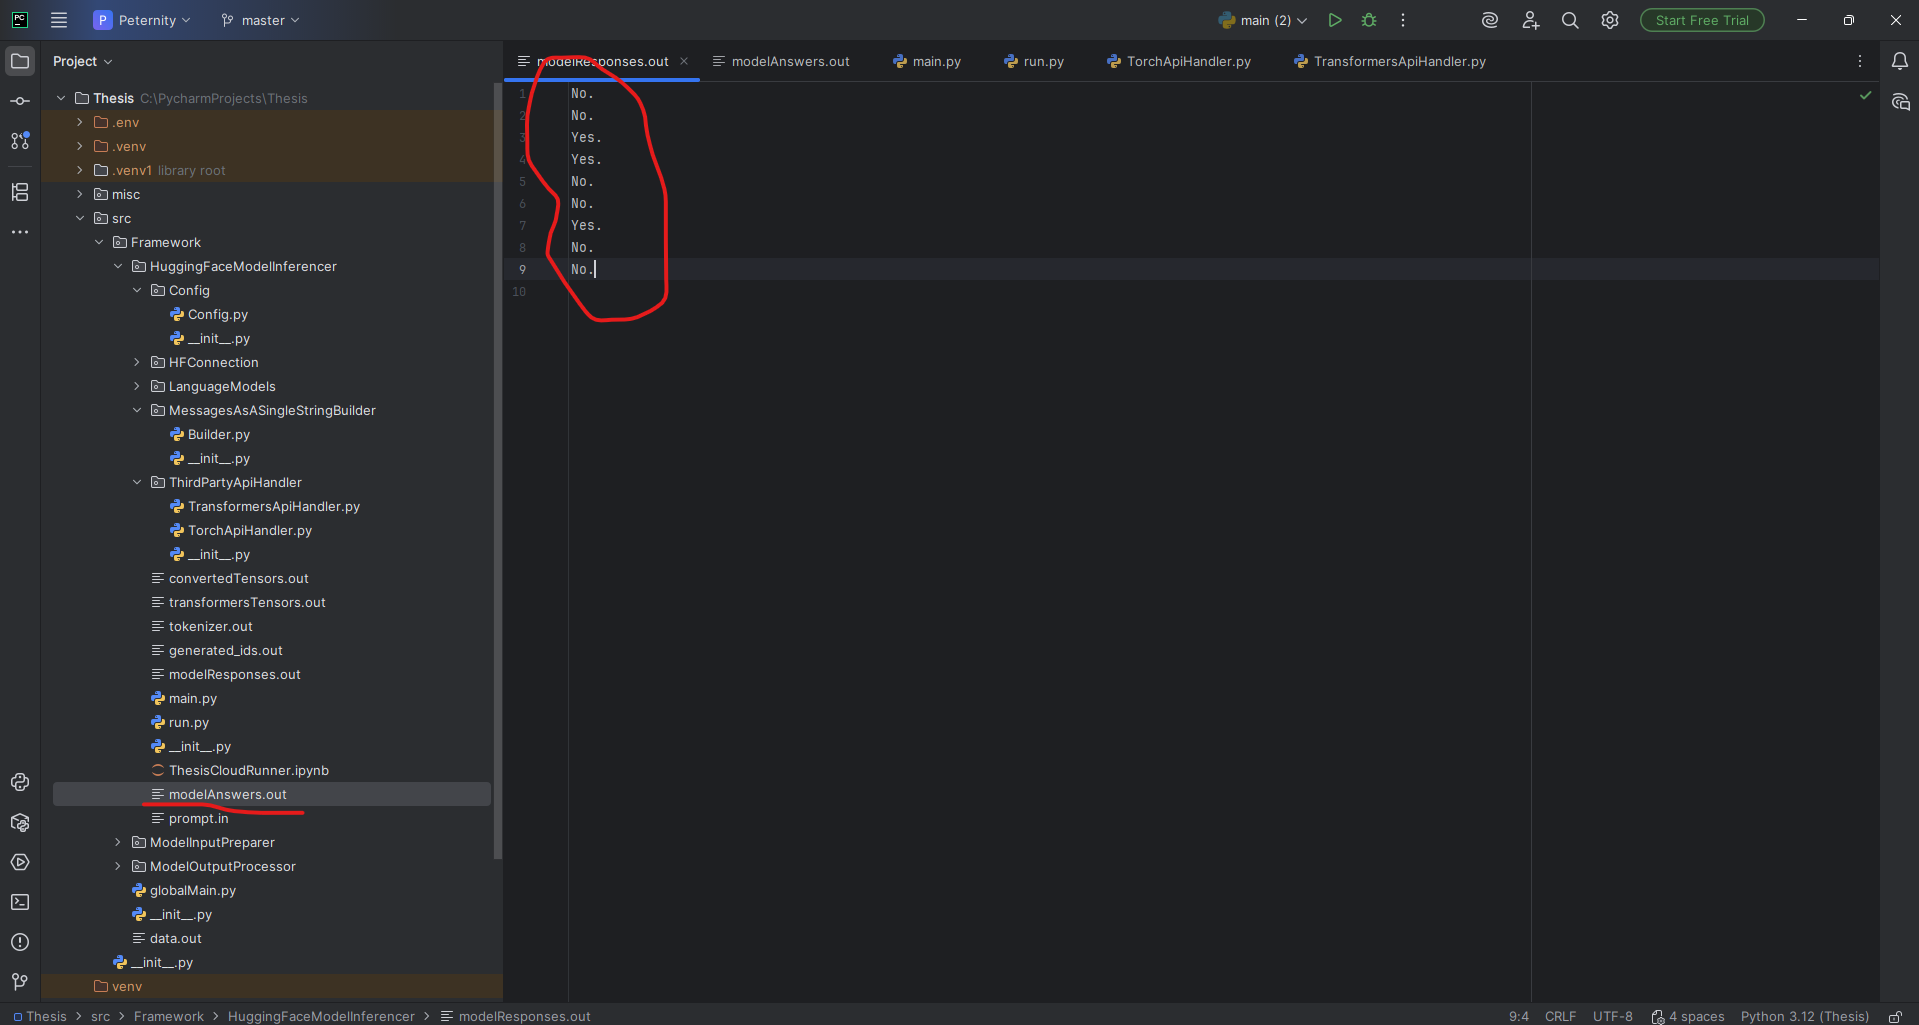
\includegraphics[keepaspectratio]{pelda}
                             \caption{Példa Válasz}
                             \label{fig:PeldaValasz}
                         \end{figure}


\chapter*{Nyilatkozat}
%Egy üres sort adunk a tartalomjegyzékhez:
\addtocontents{toc}{\ }
\addcontentsline{toc}{section}{Nyilatkozat}
%\hspace{\parindent}

% A nyilatkozat szövege más titkos és nem titkos dolgozatok esetében.
% Csak az egyik tipusú myilatokzatnak kell a dolgozatban szerepelni
% A ponok helyére az adatok értelemszerûen behelyettesídendõk es
% a szakdolgozat /diplomamunka szo megfeleloen kivalasztando.


%A nyilatkozat szövege TITKOSNAK NEM MINÕSÍTETT dolgozatban a következõ:
%A pontokkal jelölt szövegrészek értelemszerûen a szövegszerkesztõben és
%nem kézzel helyettesítendõk:

\noindent
Alulírott Fábián Bernát, programtervező informatikus BSc szakos hallgató, kijelentem, hogy a dolgozatomat a Szegedi Tudományegyetem Informatikai Intézet Számítógépes Algoritmusok és Mesterséges Intelligencia Tanszékén készítettem, a programtervező informatikus BSc diploma megszerzése érdekében.

Kijelentem, hogy a dolgozatot más szakon korábban nem védtem meg, saját munkám eredménye, és csak a hivatkozott forrásokat (szakirodalom, eszközök, stb.) használtam fel.

Tudomásul veszem, hogy szakdolgozatomat / diplomamunkámat a Szegedi Tudományegyetem Informatikai Intézet könyvtárában, a helyben olvasható könyvek között helyezik el.

\vspace*{2cm}

\begin{tabular}{lc}
	Szeged, \today\
	\hspace{2cm} & \makebox[6cm]{\dotfill} \\
	             & aláírás              \\
\end{tabular}

\vspace*{4cm}




\chapter*{Köszönetnyilvánítás}
\addcontentsline{toc}{section}{Köszönetnyilvánítás}

Ezúton szeretnék köszönetet mondani a családomnak, barátaimnak, tanítóimnak, tanáraimnak és egyetemi tanáraimnak, akik végigkísértek utamon és támogattak tanulmányaim alatt. Köszönetet szeretnék továbbá nyilvánítani szüleimnek, testvéreimnek és barátaimnak, hogy mindenben támogattak.

Végül, de nem utolsó sorban köszönetet szeretnék mondani \textbf{témavezetőmnek, Berend Gábornak}, hogy konzulensként és témavezetőként segített a szakdolgozatom megírásában.


%% Az itrodalomjegyzek keszitheto a BibTeX segedprogrammal:
%\bibliography{diploma}
%\bibliographystyle{plain}
\bibliographystyle{plainnat}
\bibliography{references}
[1] Mohammad Taher Pilehvar és Jose Camacho-Collados. „WiC: the Word-in-Context
Dataset for Evaluating Context-Sensitive Meaning Representations”. Proceedings
of the 2019 Conference of the North American Chapter of the Association for
Computational Linguistics: Human Language Technologies, Volume 1 (Long and
Short Papers). Szerk. Jill Burstein, Christy Doran és Thamar Solorio. Minneapolis,
Minnesota: Association for Computational Linguistics, 2019. jún., 1267–1273. old.
DOI: 10.18653/v1/N19-1128. URL: https://aclanthology.org/
N19-1128/.
[2] Michael E. Lesk. „Automatic Sense Disambiguation Using Machine Readable Dictionaries: How to Tell a Pine Cone from an Ice Cream Cone”. Proceedings of the
5th Annual International Conference on Systems Documentation (SIGDOC ’86).
New York, NY, USA: ACM, 1986, 24–26. old. URL: https://dl.acm.org/
doi/10.1145/318723.318728.
[3] Paul-Edouard Sarlin és tsai. SuperGlue: Learning Feature Matching with Graph Neural Networks. 2020. arXiv: 1911.11763 [cs.CV]. URL: https://
arxiv.org/abs/1911.11763.
[4] Alex Wang és tsai. SuperGLUE: A Stickier Benchmark for General-Purpose Language Understanding Systems. 2020. arXiv: 1905.00537 [cs.CL]. URL: https:
//arxiv.org/abs/1905.00537.
[5] Wei-Lin Chiang és tsai. Chatbot Arena: An Open Platform for Evaluating LLMs
by Human Preference. 2024. arXiv: 2403 . 04132 [cs.AI]. URL: https :
//arxiv.org/abs/2403.04132.
[6] Springboard. OpenAI GPT-3: Everything You Need to Know. 2023. URL: https:
//www.springboard.com/blog/data-science/machine-learninggpt-3-open-ai/.
[7] The Verge. The New York Times prohibits using its content to train AI models. 2023.
URL: https://www.theverge.com/2023/8/14/23831109/thenew-york-times-ai-web-scraping-rules-terms-of-service.
[8] Eli Tan. „When the Terms of Service Change to Make Way for A.I. Training”. The
New York Times (2024. jún.). URL: https://www.nytimes.com/2024/
06/26/technology/terms-service-ai-training.html.
[9] Thomas Wolf és tsai. „HuggingFace’s Transformers: State-of-the-art Natural Language Processing”. arXiv preprint arXiv:1910.03771 (2019). URL: https : / /
arxiv.org/abs/1910.03771.
[10] Ari Holtzman és tsai. „The Curious Case of Neural Text Degeneration”. Proceedings of the 8th International Conference on Learning Representations (ICLR).
2020. arXiv: 1904 . 09751. URL: https : / / arxiv . org / abs / 1904 .
09751.
[11] Gábor Berend. 11\_phi.ipynb. https://colab.research.google.com/
drive/1GQRiTDNWwNPP\_PPARYd1swY1Oiai9Ey\_. Google Colab jegyzetfüzet. 2025. (Elérés dátuma 2025. 05. 23.).
[12] Microsoft. Phi-4-mini-instruct. https://huggingface.co/microsoft/
Phi-4-mini-instruct. 2023.
[13] Google. Gemma-2-2b-it. https://huggingface.co/google/gemma2-2b-it. 2023.
[14] Qwen. Qwen1.5-1.8B-Chat. https://huggingface.co/Qwen/Qwen1.
5-1.8B-Chat. 2023.
[15] Steven Bird és Edward Loper. „NLTK: The Natural Language Toolkit”. Proceedings of the ACL Interactive Poster and Demonstration Sessions. Barcelona, Spain:
Association for Computational Linguistics, 2004. júl., 214–217. old. URL: https:
//aclanthology.org/P04-3031/.
[16] George A. Miller. „WordNet: A Lexical Database for English”. Human Language
Technology: Proceedings of a Workshop held at Plainsboro, New Jersey, March
8-11, 1994. 1994. URL: https://aclanthology.org/H94-1111/.
[17] Tim Peters. PEP 20 – The Zen of Python. https://peps.python.org/
pep-0020/. Python Enhancement Proposal. 2004.
[18] Samuel Oloruntoba és Anish Singh Walia. SOLID: The First 5 Principles of Object
Oriented Design. 2024. ápr. URL: https : / / www . digitalocean . com /
community / conceptual - articles / s - o - l - i - d - the - first -
five-principles-of-object-oriented-design.
[19] OpenAI. OpenAI API Documentation Overview. 2025. URL: https://platform.
openai.com/docs/overview.
[20] Anthropic. Client SDKs - Anthropic API. https://docs.anthropic.com/
en/api/client-sdks. 2025.
[21] Alessandro Raganato és tsai. XL-WiC: A Multilingual Benchmark for Evaluating Semantic Contextualization. 2020. arXiv: 2010 . 06478 [cs.CL]. URL:
https://arxiv.org/abs/2010.06478.
[22] Anna Breit és tsai. WiC-TSV: An Evaluation Benchmark for Target Sense Verification of Words in Context. 2021. arXiv: 2004.15016 [cs.CL]. URL: https:
//arxiv.org/abs/2004.15016.


%VAGY "kézzel" a következõ módon:

\begin{thebibliography}{9}
%10-nél kevesebb hivatkozás esetén

%\begin{thebibliography}{99}
% 10-nél több hivatkozás esetén

\addcontentsline{toc}{section}{Irodalomjegyzék}

%Elso szerzok vezetekneve alapjan ábécérendben rendezve.


%folyóirat cikk: szerzok(k), a folyóirat neve kiemelve,
%az evfolyam felkoveren, zarojelben az evszam, vegul az oldalszamok es pont.
\bibitem{Gischer}
J. L. Gischer,
The equational theory of pomsets.
\emph{Theoret. Comput. Sci.}, \textbf{61}(1988), 199--224.

%könyv (szerzo(k), a könyv neve kiemelve, utana a kiado, a kiado szekhelye, az evszam es pont.)
\bibitem{Pin}
J.-E. Pin,
\emph{Varieties of Formal Languages},
Plenum Publishing Corp., New York, 1986.





\end{thebibliography}

\chapter*{Elektronikus mellékletek}
\addcontentsline{toc}{section}{Nyilatkozat}

\begin{itemize}
\item A keretrendszeren GitHubról a\\ \href{https://github.com/Fabbernat/Thesis}{GitHub/Fabbernat/Thesis}\\ repozitóriumban található.

\item A szakdolgozat pdf forráskódja a \href{https://github.com/Fabbernat/Thesis-paper}{GitHub/Fabbernat/Thesis-paper}\\ repozitóriumban található.

    \item
\label{att:colab}
A modelleket futtató Google Colab jegyzetfüzetem (elavult):
\href{https://colab.research.google.com/drive/1yA8IAd5z2oreKUXha-16Du2YrNhemNiU?usp=sharing}{ezen a linken}  található.

\item A nyelvi modellek tesztelésének és kiértékelésének régi eredményei a
\href{https://docs.google.com/spreadsheets/d/1y49lg52LHVFmTom-0ibCqYqWA1pKKhiUny-Pf3KVTIg/edit?usp=sharing}{Generative Language Models}
táblázatban tekinthető meg.
\end{itemize}


\end{document}
